\begin{section}{Framework Tools}

\subsection{PostSharp}
PostSharp (Aspekt orientierte Programmierung):
Dieses Tool wird verwendet, um eigene Aspekte bzw. Attribute schreiben zu können. Konkret wurde es für das Exception Handling in der DAL Schnittstelle verwendet. Das Attribut „DaoExceptionhandlerAttribute“ fängt eine auftretende Exception (z.B. bei einer Datenbank Abfrage) ab und wrappt diese in das generische DAOResponse Objekt. In weiterer Folge wird dieses Konzept noch näher erläutert. Nachfolgend wird beschrieben wie PostSharp in Visual Studio eingebunden werden kann. Für die Ausführung wird eine Free-Lizenz verwendet.

\subsubsection{Installation}
Unter folgendem Link kann PostSharp runtergeladen werden.\newline
\url{https://www.postsharp.net/download}

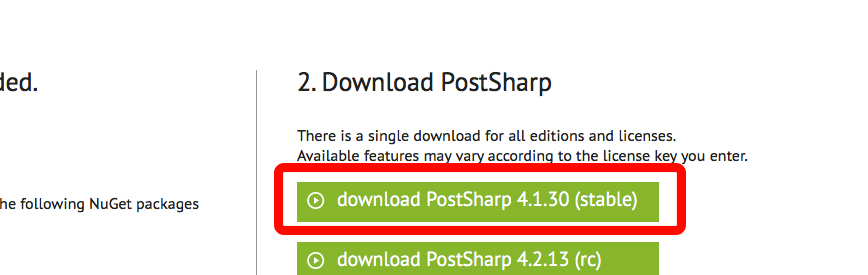
\includegraphics[angle=0, scale=0.45]{./img/postsharp1.jpg}
\FloatBarrier

\subsubsection{Registrierung / Account anlegen}
Um PostSharp im PostCompile Ablauf verwenden zu können, wird wie unten dargestellt, eine Freie Lizenzregistrierung benötigt.

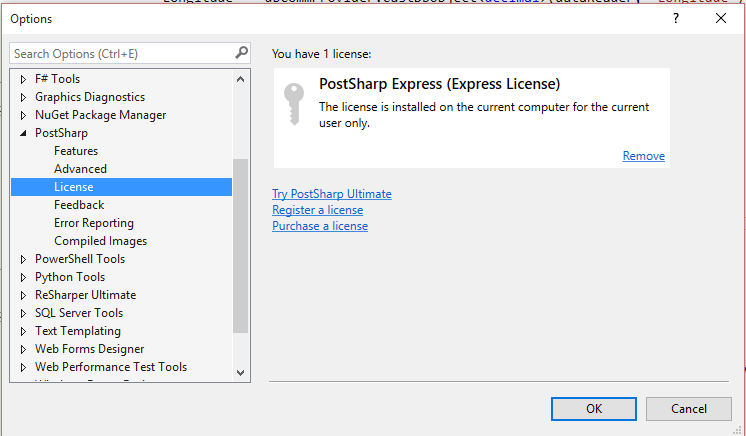
\includegraphics[angle=0, scale=0.45]{./img/postsharp3.jpg}
\FloatBarrier

		
\end{section}